%%%%%%%%%%%%%%%%%%%%%%%%%%%%%%%%%%%%%%%%%%%%%%%%%%%%%%%%%%%%%%%%%%%%%%%%%%%%%%%%
%2345678901234567890123456789012345678901234567890123456789012345678901234567890
%        1         2         3         4         5         6         7         8

\documentclass[letterpaper, 10 pt, conference]{ieeeconf}  % Comment this line out
                                                          % if you need a4paper
%\documentclass[a4paper, 10pt, conference]{ieeeconf}      % Use this line for a4
                                                          % paper

\IEEEoverridecommandlockouts                              % This command is only
                                                          % needed if you want to
                                                          % use the \thanks command
\overrideIEEEmargins
% See the \addtolength command later in the file to balance the column lengths
% on the last page of the document

\usepackage[utf8]{inputenc}
\usepackage[T1]{fontenc}
\usepackage{cite}
\usepackage{hyperref}
\usepackage{graphicx}

% The following packages can be found on http:\\www.ctan.org
%\usepackage{graphics} % for pdf, bitmapped graphics files
%\usepackage{epsfig} % for postscript graphics files
%\usepackage{mathptmx} % assumes new font selection scheme installed
%\usepackage{mathptmx} % assumes new font selection scheme installed
%\usepackage{amsmath} % assumes amsmath package installed
%\usepackage{amssymb}  % assumes amsmath package installed

\title{\LARGE \bf
Detection and Analysis of
Exoplanets using Machine Learning
Techniques
}

%\author{ \parbox{3 in}{\centering Lance Dacy*
%         \thanks{*Use the $\backslash$thanks command to put information here}\\
%         Faculty of Electrical Engineering, Mathematics and Computer Science\\
%         University of Twente\\
%         7500 AE Enschede, The Netherlands\\
%         {\tt\small h.kwakernaak@autsubmit.com}}
%         \hspace*{ 0.5 in}
%         \parbox{3 in}{ \centering Thomas Karba**
%         \thanks{**The footnote marks may be inserted manually}\\
%        Department of Electrical Engineering \\
%         Wright State University\\
%         Dayton, OH 45435, USA\\
%         {\tt\small pmisra@cs.wright.edu}}
%}

\author{Lance Dacy$^{1}$, Aurian Ghaemmaghami$^{2}$, Aniketh Vankina$^{3}$, and Jamie Vo$^{4}$% <-this % stops a space
}

\begin{document}

\maketitle
\thispagestyle{empty}
\pagestyle{empty}

%%%%%%%%%%%%%%%%%%%%%%%%%%%%%%%%%%%%%%%%%%%%%%%%%%%%%%%%%%%%%%%%%%%%%%%%%%%%%%%%

\begin{abstract}

The Earth's population continues to grow at a steady rate. The natural resources on Earth are in limited supply. The need to find other worlds that could contain life becomes more focused and intense in the past few years. Scientists desire to find exoplanets that have the features similar to Earth for sustaining life, not only for curiosity sake, but for potential new places for humans to thrive. The data collected over the centuries is so large that filtering the data becomes problematic. With new technologies that use a machine's processing power, data science methods could help scientist evaluate this data and its patterns to narrow down exoplanets that could sustain life as we know it. The data needed to model these exoplanets need to be easily consumed; this project will focus on the viability of deploying cloud data stores specifically to aid in exoplanet modeling.

\end{abstract}


%%%%%%%%%%%%%%%%%%%%%%%%%%%%%%%%%%%%%%%%%%%%%%%%%%%%%%%%%%%%%%%%%%%%%%%%%%%%%%%%
\section{Introduction}

Are we alone in the Universe? That is an age-old question that humans having been striving to answer since we first identified that our planet is simply a small part of a larger whole. Earth appears to be one of the planets in the whole Universe that has just the right ingredients to host life. Or is it? The science continues to explore that question "Are we alone?" and have developed a systematic approach of the course of centuries to help compile data that might just answer that question. 

We live in a technology age where it is feasible to gather mounds of data about our Universe. Even better, we live in a technology age where computers can assist in stitching that data together to help find the patters that point us in the right direction for an answer. Our Data Science Team joins the ranks of numerous scientist to help analyze the  myriad data gathered from the Universe to find the building blocks essential to host life as we know it. Given the quest for life as we know it, scientist narrow down the building blocks to a simple acronym called CHNOPS. CHNOPS stands for Carbon, Hydrogen, Oxygen, Phosphorus, and Sulfur. These are the base elements believed to provide the building blocks for living organisms. Finding a place in the Universe that contains these elements is much like finding a needle in a haystack.

Aside from the fact that the human race has a quest to find others in the Universe, there is also another need that needs to be sustained. We will eventually consume all the natural resources on this precious Earth. The Earth's population continues to grow at a rate of 1.05\%~\cite{BASAK2020100335}. 

\begin{figure}
	\centering
	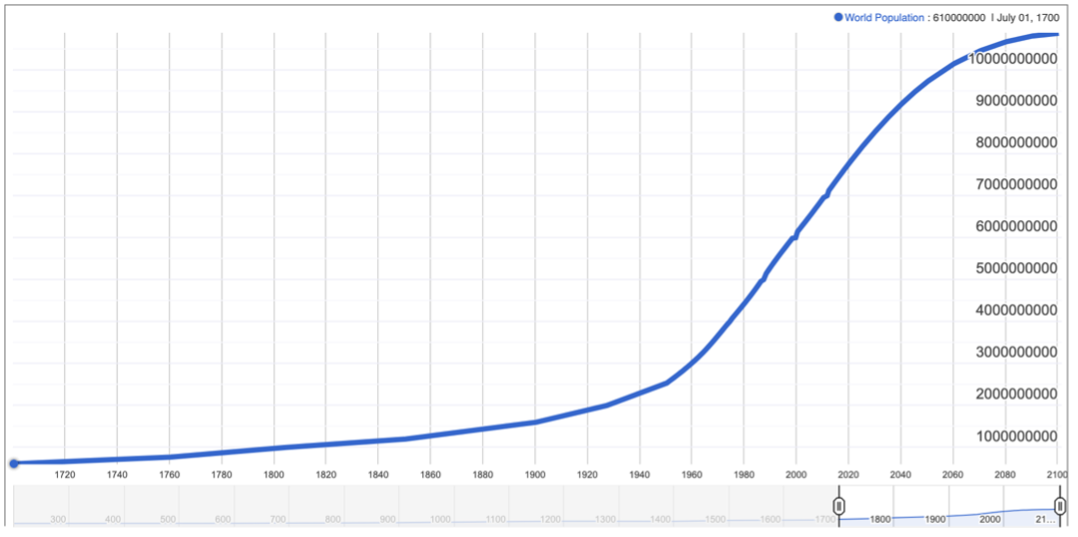
\includegraphics[width=0.7\linewidth]{Images/WorldPopulation}
	\caption[World Population from 1700's to Present Day]{World Population: Past, Present, and Future. The graph displays the population increase from the 1700's to present day.}~\cite{PopulationClock202007}
	\label{fig:worldpopulation}
\end{figure}

The planet’s resources are expected to cap at nearly 8 billion people. The Earth currently inhabits 7.8 billion as of July 2020. Earth’s estimated timeline to maintain complex life is anticipated to cease to exist as early as 1.5 billion years. Apart from discovering life at a habitable planet, space exploration allows humankind to gain a greater understanding of the cosmos and potentially answer the question of, “Is there life beyond Earth?”~\cite{ScienceMissionDirectorate2020} and more importantly, could we catapult the human race to this newfound habitable planet.

As mentioned earlier, the good news is that we have mounds of data that have been collected over the last centuries. What is lacking is a good way to determine patterns in all of the data with computational cycles of the human brain. NASA has collected Kepler data that is a repository of the type of information needed to answer some of the questions of  the human race. Unfortunately, as with most big data systems, the repository is data rich, but information poor. It is. becoming increasingly difficult to filter the data to meaningful levels. The data contains information on image sources, light measures, and gravity among other things. In conjunction with the volume of data is the unknown requirements that confirm if a planet is habitable, analyzing the parameters pouring in to confirm a planet, and understanding the cosmic web that connects the galaxies which hold potential habitable planets. 

This project's goal is aimed at answering the following problem: Based on the myriad data available about space exploration, is it possible to provide an estimate of the number of other exoplanets in the Universe that are able to maintain life as we know it? In addition, could a repeatable hosted data center be built that allows for the community to consume and build algorithms for this specific purpose; easing the issue of data filtering? The main contributions to this paper are mentioned  in the references section which supports the understanding of the science behind this data. In the early stages of the paper, the team will discuss the motivation behind the problems statement and then continue on into the methodologies considered. More focus will be aimed at the hosting and replication of the data using Amazon Web Services (AWS) than the actual algorithms used to determine habitual planets. Nonetheless, the team will demonstrate a few algorithm techniques to prove out the hosting platform and its feasibility. The team will then explore methodologies in deep learning and machine learning that are widely used in the application of exoplanet scientific research. This will entail creating a working model to detect exoplanet feasibility based on configurable parameters set by the scientists and showcase the platform of data that will be served against those models. The team will then move on to the various milestones of the project which are the ability to collect the data, store the data in the Cloud (AWS), configure ETL processes that can be consumed, and then deploy a few machine learning models that will consume the data store.

\section{Motivation}

Based on algorithms and programs provided in research, it is possible to reign in the available data and provide a predictable and repeatable method to determine whether exoplanets in the Universe are habitable. Having an affinity of space, data science, and the hosting of large data sets provides the background for such experiments to thrive. As mentioned in the Introduction, the Astronomy data community find themselves data rich, information poor. While mounds of data exists, there is so much that even filtering the data is problematic. The best solution would be to find ways to federate the data to specific fields of studies. If a scientist is trying to determine where the next Super Nova will occur, they need specific pieces of data. Another scientist looking for the best environments for nebulae will look at another set of data. The mission of this project is to find what data elements would be best suited for helping scientist determine exoplanets and find a predictable and repeatable method to host and consume that data. 

The only race on Earth is the human race, we must band together, using all technologies available to help sustain the human race. Earth is on borrowed time. Population growth and natural resource consumption will end tragically for Earth at some point in the future. Humans must invest in ways to either minimize natural resource consumption or look for other parts of the Universe that we could colonize. Armageddon comes in many forms: climate breakdown, asteroid strike, zombie apocalypse, and so on. There are scientist that choose to use the Copernican Principle with statistics to figure out how long anything will last. We could use this to determine within a 95\% confidence how long humans will be around. Right now, that number is somewhere between 5,130 to 7.8 million years if you assume that humans have been around for about 200,000 years~\cite{Koehrsen2018}. This is in close correlation with the mean duration of a mammal species; which is about 2million years. 

\begin{figure}
	\centering
	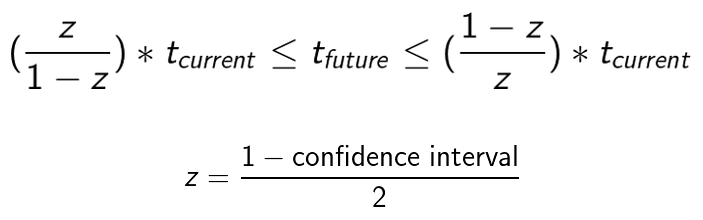
\includegraphics[width=0.7\linewidth]{Images/Formula}
	\caption[The Copernican Lifetime Equation]{The Copernican Lifetime Equation}~\cite{Koehrsen2018}
	\label{fig:formula}
\end{figure}

While the motivation might not be there for our current generation; technology evolves as stepping stones from generation to generation. The need to support scientists in taking the next big steps of finding exoplanets is now. The technology is ripe, the desires are there, all that is needed are tools to move us in the right direction. The next question in generations to come might be, "how do we get to said exoplanet", but technology isn't really at a point to answer that question yet. The first step is to equip scientists with data techniques that allow them to pin point areas that could provide colonization options. The sooner we do this, the sooner we can move on to the next stepping stone of technology needs.

\section{Methodology}

Machine learning techniques along with Deep Learning are widely used in application for various exoplanet scientific research. One thing that is quite uncertain is the number of actual planets that exist outside our own solar system. There are various techniques that can be utilized to help us with this detection. Before delving into the techniques that can be used for prediction, data management needs to be touched upon. When it comes to any analysis, data is required. However, where the data is stored can be a huge concern. Traditional databases go a long way, but in order to do efficient and thorough work, it is important to store this information in a secure and accessible way. Cloud technology makes hosting this type of data easy. By utilizing Amazon Web Services (AWS) S3 and RDS (Relational Database Service) services this task can be accomplished. The benefits of having this storage and data management power, is scalability as well as quality ~\cite{CloudDataManagement}. Especially when working with data that is ever growing in the "Planet/Space" field, scalability is huge. 

As touched upon, Amazon's S3 service helps with storage of clean and robust data. The option to expand storage as well as version control will alleviate any burden of mismatched data. Traditional storage services like DropBox are great for storing data but not really helpful in terms of version control. This can be done in S3 services. Performance is also an important factor when it comes to manipulation. Amazon S3 is ideal when it comes to fast delivery times with the options of image and video rendering ~\cite{AmazonS3}. This might be fruitful when more renders of exoplanets can be collected. On top of its power to store data, analysis can be done with in-place querying functionality and there are many third party tools integrated that can be used ~\cite{AmazonS3}. Overall, AWS S3 will be the most leveraged service for its all around capabilities.

AWS also offers RDS services that can be further used for storage and querying. Similar to S3, Amazon RDS has many of the same characteristics but is tailored towards the database realm. Some prime attributes include Scalability, Availability, Vertical Scalability, Horizontal Scalability, and Performance ~\cite{AWSRDSBenefits}. How effectively this service can be utilized in terms of this project will be discussed further, as the primary winner will be S3 services. 

Additionally throughout this paper, it is also essential to create a models that can detect whether or not life can be accommodated in these various exoplanets. One of the main Machine Learning methods that can be utilized that is beneficial to this topic is classification. Classification models are one of the key supervised techniques that can be leveraged in exoplanet detection. Based on our research from various literature the following methods would be best suited for this type of work. 

In Cameron et. al ~\cite{MLApproachesExoPlanets} there were numerous classification techniques that were used for exoplanet detection. The following classification techniques were used: Support Vectors, Linear Support Vector, K-Nearest Neighbors, Random Forest, and finally Logistic Regression. Ideally, these supervised techniques will be the easiest and more suitable to be run. This can be due to the fact that these techniques have been in practice and are some staple techniques. The research and performance will be discussed more detailed in the ML milestones section later on this paper.

\section{Milstones-Data Collection}

The data was collected from NASA's exoplanet site which contains 287 columns, ranging from the planet's name to data concerning the galaxy where exo-planet lives in. Originally pulled from an API, due to the recent changes in the NASA site, the data can be exported to a csv. All data in the table are reviewed by a team of astronomers, verifying its accuracy. The data is collected through a number of means, including various telescopes (such as the kepler mission) or satelites such as the TESS, which is part of the NASA's explorer program. The data also includes focuses on the host stars of the planets, for deeper understandings of how the planet's access to sunlight, temperature, etc.~\cite{nasaExoplanetArchive}. 

\section{Milestones-Data Storage in the Cloud}

Exoplanet research and big data tend to go hand in hand. With so much new information being ingested every day, it is important to understand the use cases and benefits when it comes to storing and accessing that information for action-related purposes. As denoted in our methodology, AWS S3 buckets provide the level of seamless integration and accessibility that will be applicable to our exoplanet research at hand. Amazon S3 also provides use cases in scalability and security. Having the data available is one need but making sure those data objects are secure to only the end users is another caveat that Amazon S3 alleviates ~\cite{AmazonS3}. The tool also provides a lot of hands-off access management and encryption features which allow the user to block certain access points to ensure the integrity of the data isn't compromised. Lastly, as mentioned prior, query performance within S3 is a dire need as we ingest NASA's exoplanet data. Our goal is to leverage and select subsets of data objects to help eliminate unneeded noise hat may cause the query to take longer to process. Given these advantages, this research will rely heavily on the hosting functionality of S3 as we socialize out the ETL pipeline.

\section{Milestones-ETL}

It is important to note that setting up a robust ETL process is crucial as we are pulling in large amounts of data surrounding exoplanet scientific research. Such data volumes make it extremely hard for an average individual to both download and process this data on a quick time scale. ETL operations in short are designed to essentially collect, read, and migrate data across different platforms from various data structures. Usually, an ETL job will read in the data from a data source, transform the data given the nature of your problem and then writes the results to a source ready for ingestion. Given the nature of this research, AWS provides multiple ETL tools and operations to help with processing, scaling, computing, and parallelization ~\cite{AmazonGlue}.

As stated in the methodology, a goal is to leverage tools like S3 and Amazon RDS in a collaborative fashion that will allow for scalable, faster data integration with little to no responsibility on the infrastructure side for the user. AWS Glue is a server-less data integration service that makes it easy to discover, prepare, and combine data for analytics, machine learning, and application development ~\cite{AmazonGlue}. This tool has been leveraged in other exoplanet studies where AWS Glue was utilized to allow astronauts  the ability to download full file space images in a matter of seconds without it being computationally expensive or taking too long to download ~\cite{AmazonGlueUsage}. AWS Glue also integrates well with Amazon S3 and RDS providing a full catalog to find data across multiple sources as new data becomes available and ingested. If the end user already has a set database and Amazon RDS is not needed, then AWS Glue can integrate with the database through an EC2 instance to start the data ingestion process.

Let’s say there is a scenario where cost is an important factor to consider and leveraging tools like AWS Glue isn’t achievable. Given the nature of our research, we can still utilize AWS EC2, S3, and Lambda functions to achieve our goals from an ETL standpoint. This will still allow the flexibility of doing large data manipulations without having to finance an infrastructure. In a nutshell, this research would start in phases for the ETL process. First, our research will leverage pulling our necessary data from NASA's API while running on an EC2 instance. Next, there is an orchestration of lambda functions that can then be initiated to run alongside your ETL structure to complete jobs that you have set for it to trigger. AWS Lambda functions are increasingly crucial for a task like this because you can manually set multiple jobs with different Lambda functions to help with the transformation and manipulation of your data. This flexibility can also open up new strategies to incorporate parallelization within your lambda functions to help with performance and efficiency as new data becomes available ~\cite{AmazonLambda}. Lastly, the data will be hosted on S3 where it can be easily managed, accessed, and queried for our research needs.

\section{Milstones-Machine Learning Models}

As briefly talked about in the methodology section, one of the research consisted of multiple classification techniques being used. The overall results for two of the models SVC and RFC were 93\% and 94\% respectively ~\cite{MLApproachesExoPlanets}. The results were great and we can tell that these techniques are viable for a classification tasks that are required. However, since the data will be hosted on cloud services, there are third party and native tools that Amazon offers out the box.

In a popular and ever growing field such as Machine Learning, AWS makes it easy to create and scale our ML models. One such software that Amazon offers is called AML (Amazon Machine Learning). The great part about this tool is that it is skill level agnostic, meaning people of all skill levels can pick it up fairly easy ~\cite{PopularMLSoftware}. As specified above, the common types of models that will be ran is classification. AML supports three types of models: multi-class classification, binary classification, and regression ~\cite{PopularMLSoftware}. This is a great tool that can be leveraged for the exoplanet analysis. It is definitely the tool that should be utilized since the data will be stored in S3.

The other service that is highly publicized is Amazon SageMaker. There is a reason that this one of the fastest growing services because many companies and BI teams are moving over to the cloud. According to AWS website, SageMaker can increase productivity times 10 and also the cost reduction (compute power allocation) ~\cite{AmazonSagemaker}. This tool can be useful for planet analysis because of its ease of use as well as speed. It will make scaling the models much quicker. 

The above are some of the milestones and tasks that would ideally be accomplished. These existing tools will play a huge role in helping us scale and make predictions.

\section{CONCLUSIONS}

While determining whether extraterrestrial life exists apart from planet Earth is still in question, there is no wonder of whether or not humans will be able to continue existence on earth to the end of time. NASA's data collection has grown to a point where its no longer human readable, examinable, or on a scale of analysis. In order to assist with the growth levels of the information pouring in daily, methods of machine and deep learning are leveraged to assist scientists in digesting the data. 

In addition, by storing the data on cloud, such as Amazon's S3 service, this allows users to scale the data in a manageable method. In addition, data integrity and accessibility are managed through Amazon's services, preventing users from concerning themselves with network security concerns and allows focus on analysis and pattern extraction. Leveraging the many cloud services provides speed and capabilities which would not be possible on a base metal machine, elevating the experience and propelling discovery. 

\addtolength{\textheight}{-12cm}   % This command serves to balance the column lengths
                                  % on the last page of the document manually. It shortens
                                  % the textheight of the last page by a suitable amount.
                                  % This command does not take effect until the next page
                                  % so it should come on the page before the last. Make
                                  % sure that you do not shorten the textheight too much.

%%%%%%%%%%%%%%%%%%%%%%%%%%%%%%%%%%%%%%%%%%%%%%%%%%%%%%%%%%%%%%%%%%%%%%%%%%%%%%%%

\bibliography{references}{}
\bibliographystyle{IEEEtran}
\end{document}